\subsection{Game Engine design}
\label{sec:GameEngineDesign}

\noindent Spillets logik styres fra game engine, der består
af de komponenter, som modellere spillets verden og dens 
logik. Af disse komponenter er Game Controlleren, Combat Controlleren,
Room, og Player de mest essentielle.

\begin{figure}[H]
  \centering
  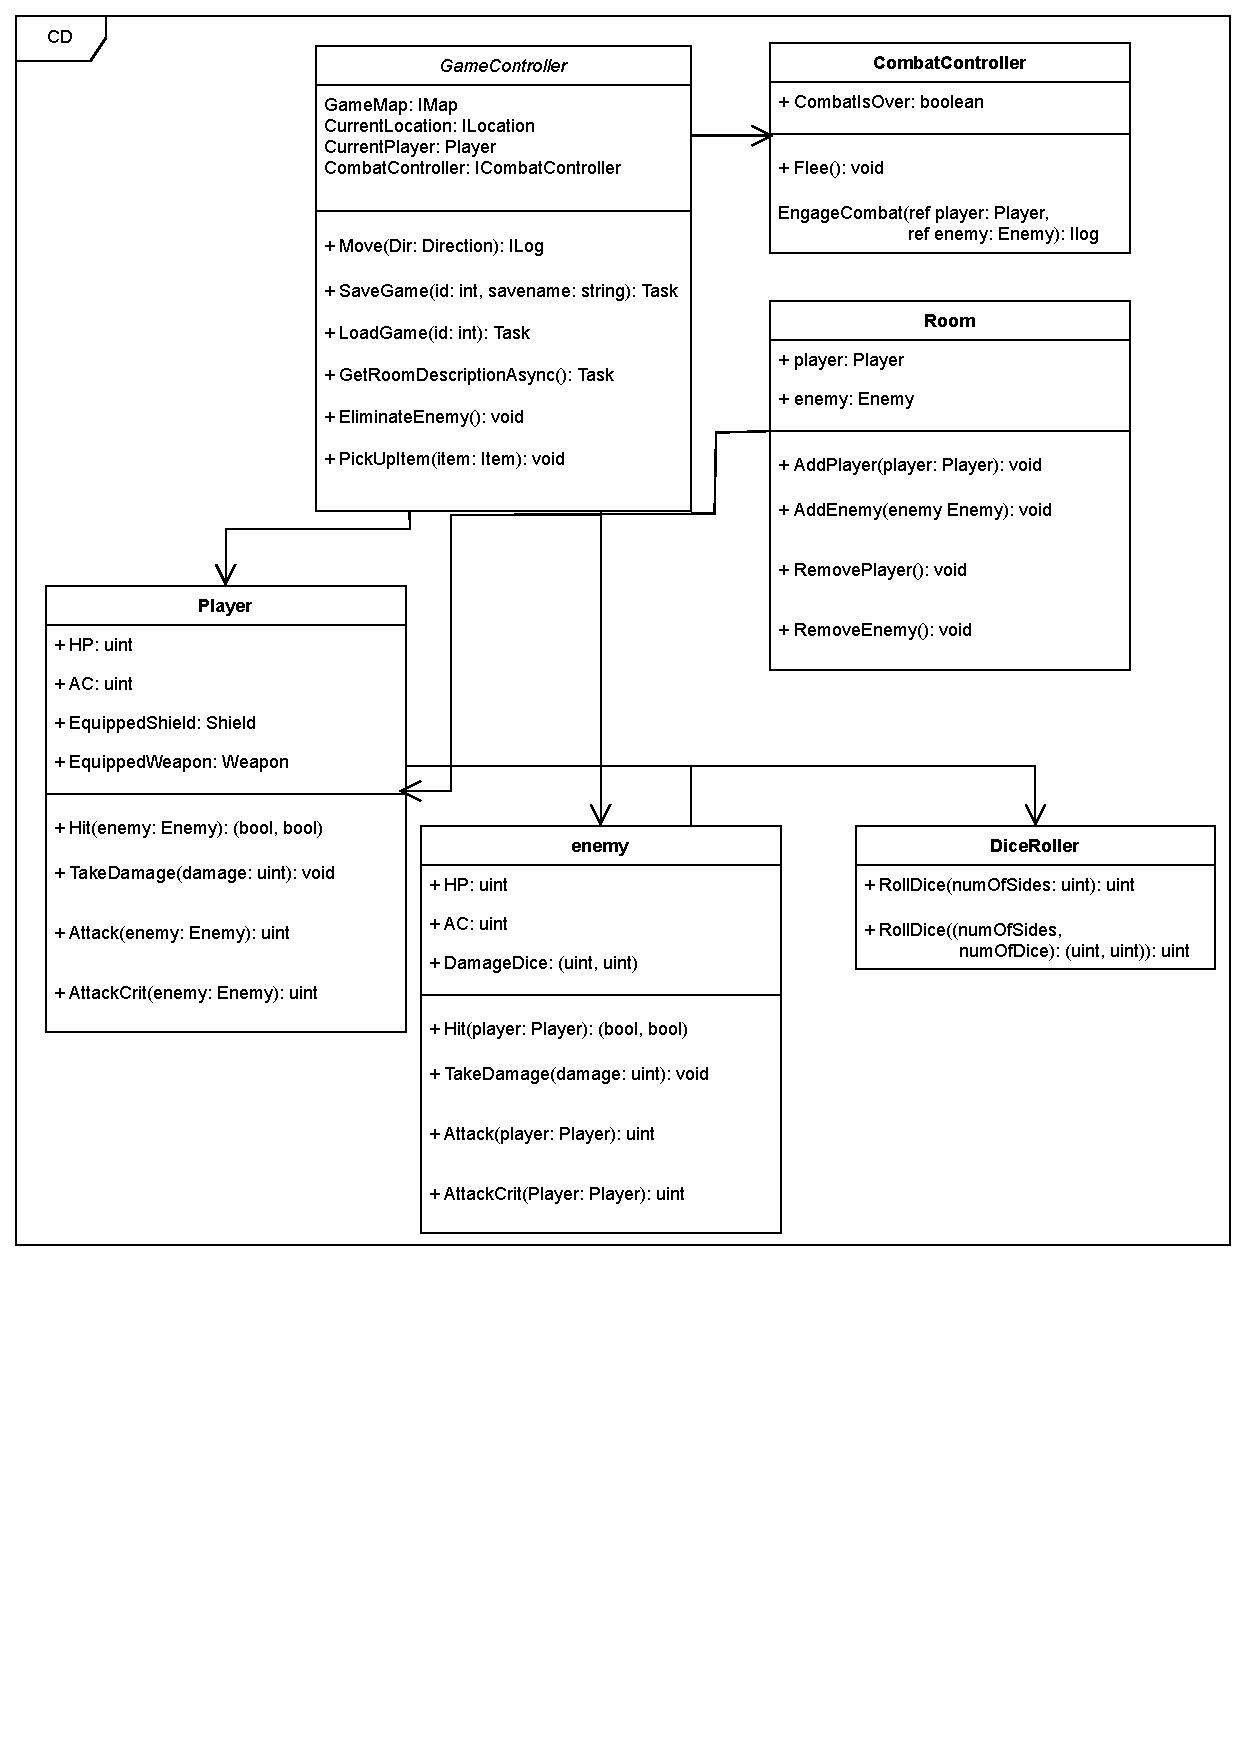
\includegraphics[width=\textwidth, trim = 0 9cm 0 0]{02-Body/Images/CoreClassDiagram.pdf}
  \caption{De vigtigste elementer af game engine og deres 
           relationer til hinanden. Der er her ikke vist 
           interfaces, men lagt fokus på de kritiske elementer
           som de er implementeret.}%
  \label{fig:CoreDiagram}
\end{figure}

\subsubsection{Game Controller}
Game Controlleren styre alle UI funktionaliteter, når brugeren
trykker på en knap, der påvirker spillets state, gøres dette
gennem game controlleren. Game controlleren instantieres når
et spil startes; hvilket danner et map \parencite[Section 10.3.1][]
{TekniskBilag}, spilleren kan navigere rundt på. 

Game controlleren tillader at spilleren kan bevæge sig mellem
spillets forskellige rum \parencite[Section 9.3.1][]{TekniskBilag} 
i overenstemmelse med spillets map layout. Skulle spilleren forsøge at
bevæge sig i en retning, der ikke er tilladt ifølge map layoutet bliver 
spilleren stående i det nuværende rum.

Skulle spilleren bevæge sig ind i et rum med et ``item'', styre 
game controlleren spillerens evne til at inteagere med ``itemet''.
Spilleren har evenen til at samle ``items'' op, og derved øge deres
stats.

I det tilfælde, at spilleren bevæger sig ind i et rum med en modstander,
giver game controlleren spilleren evnen til at bekæmpe fjenden eller
flygte fra denne. Game controlleren gør dette ved at kalde combat controlleren,
som håndtere kamp i spillet.

\subsubsection{Combat Controller}
Combat controlleren håndterer spillets logik, i det omfang det relatere sig til
kamp mellem spilleren og en fjende \parencite[Section 9.3.3][Figur 17]{TekniskBilag}.

\noindent Combat i spillet afvikles ved hjælp af flere simulerede terningekast (RNG) se dicerollern,
i \autoref{fig:CoreDiagram} der afgører både om spilleren/fjenden rammer fjenden/spilleren 
og hvor meget skade fjende/spilleren modtager. Spillets ``items'' har indflydelse
på vægtningen af disse simulerede terningekast, og kan hjælpe spilleren med at ramme og skade 
modstanderen. ``items'' kan også gøre det svære for fjenden at ramme spilleren.

Spilleren kan efter hvert sæt af terningekast vælge at forsætte kampen eller
flygte. Skulle spillerens liv nå nul, dør spilleren og spillet er færdigt.

\subsubsection{Room}
Et ``Room'' eller rum er en diskret delmængde af spillets verden, som kan indeholde
spilleren, fjender og forskellige genstande. ``Room'' er kun ansvarlig for at tilføje
og fjerne spilleren og fjender for rummet se \autoref{fig:CoreDiagram}. Ikke desto mindre
kunne spilleren ikke navigere verden uden existensen af disse diskrete områder.

\subsubsection{Player}
Spilleren karakter (PC) repræsenterer spilleren i spillet. Dette komponent er ansvarlig for at
holde styr på spillerens tilstand i spillet og giver spilleren evnen til at forsvare
sig selv i kamp. Denne simulerer en spillers forsøg på at ramme en fjende, skade en 
fjende og opdatere spilleren liv, forsvar og ``items'' undervejs i spillet 
\parencite[Section 13.3.2][]{TekniskBilag}.


\newpage
